\documentclass[13pt]{zettel}

\renewcommand{\gregor}{\put(9.2,-3.5){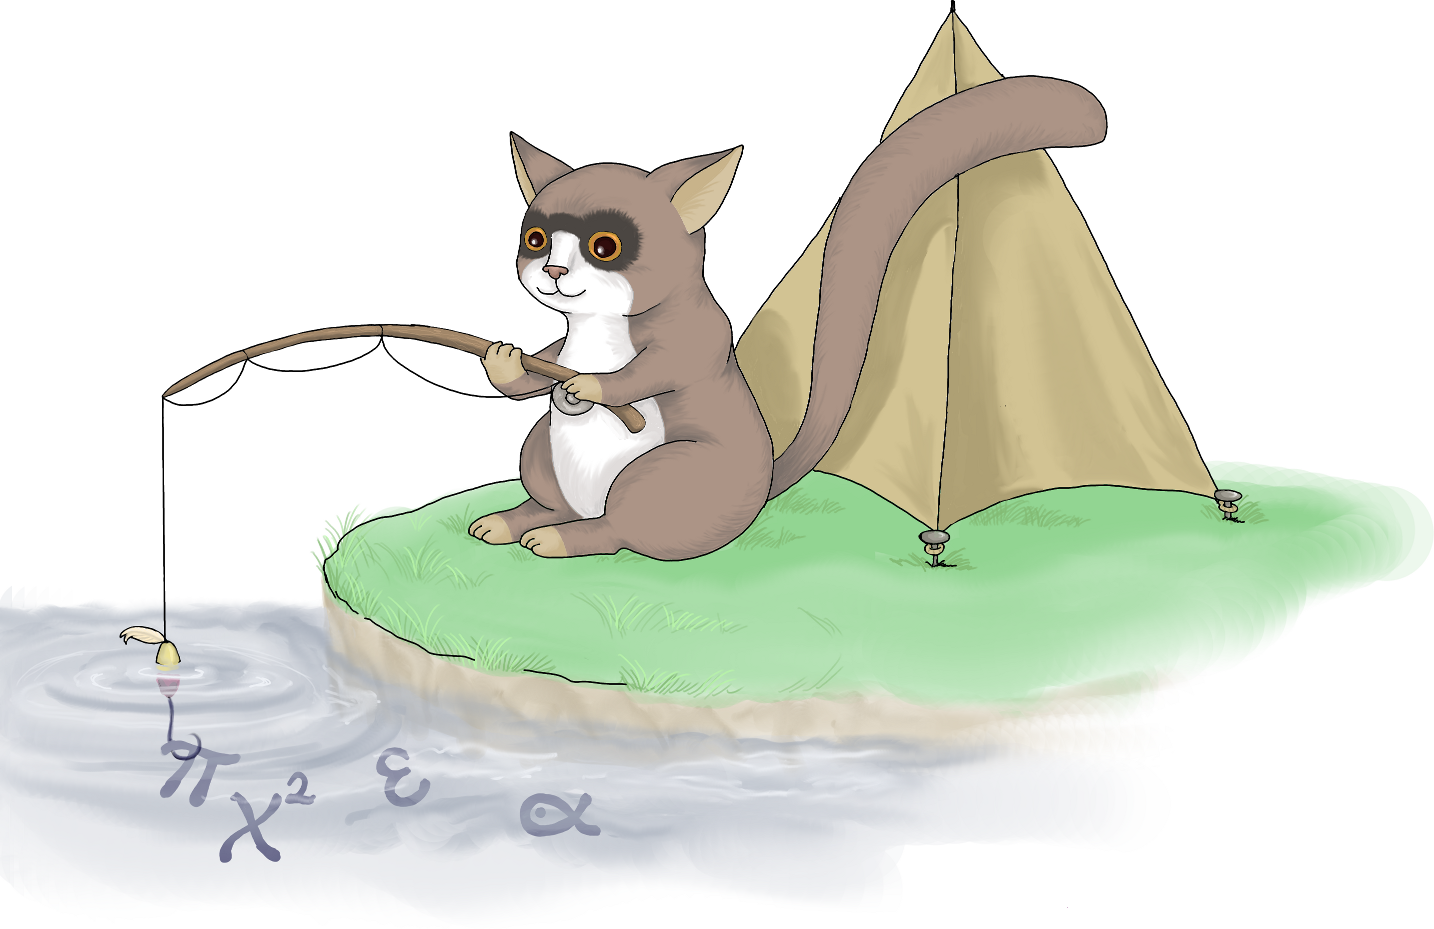
\includegraphics[scale=0.18]{campgregor}}}

\usepackage{framed}
\usepackage{enumitem}
\definecolor{shadecolor}{rgb}{.98,.98,.98}

\renewcommand{\labelitemi}{\checkbox}
\newenvironment{themabox}[1]{%
  \vspace{-0.8em}%
  \begin{enumerate}[labelindent=0pt,labelwidth=2.35cm,itemindent=0em,leftmargin=!,align=left]
    \item[\textbf{#1}]
      \begin{itemize}
}{\end{itemize}\end{enumerate}\vspace{-0.3em}}

\begin{document}

\renewcommand{\betreff}{Anmeldung zum Mathecamp des Matheschülerzirkels Augsburg}

\makeletterhead{\emph{Bitte in Druckbuchstaben ausfüllen und
bis zum 1. Juni 2015 an obige Adresse, per Fax an 0821/598-2090 oder per Mail
an
\href{mailto:mathezirkel@math.uni-augsburg.de}{mathezirkel@math.uni-augsburg.de} schicken.
Dieses Formular gibt es auch im Internet unter
\href{http://www.math.uni-augsburg.de/schueler/mathezirkel/}{http:/\!/www.math.uni-augsburg.de/schueler/mathezirkel/}.
}}

\vspace{-1.0em}

Hiermit melde ich meine Tochter/meinen Sohn verbindlich zum Mathecamp des
Mathe\-schü\-ler\-zir\-kels Augsburg vom 22. bis 28. August 2015 in
Violau an.

\vspace{-1.0em}
\doublespacing
\begin{tabbing}
  Teilnahme am: \= \kill
  Name: \> \freistLang \checkbox weiblich \checkbox männlich \\
  Adresse: \> \freistLang \\
  \> \freistLang \\
  E-Mail Eltern: \> \freistLang{} \textsc{\small (in Druckbuchstaben!)} \\
% E-Mail Kind: \> \freistLang \\
  Telefon Eltern: \> \freistLang \\
  Handy Kind: \> \freistLang \\
  Geboren am: \> \freistLang \\
  Schule: \> \freistLang \\
  Klassenstufe: \> \freistKurz{} im Schuljahr 2014/15
\end{tabbing}

\vspace{-0.8cm}
\begin{shaded}
\textbf{Notfallkontakte} Bei Bedarf sollen benachrichtigt werden (Name, Telefonnummer):
\begin{enumerate}
\item \freist{7cm},\quad\freist{7cm}
\item \freist{7cm},\quad\freist{7cm}
\end{enumerate}
\end{shaded}

\enlargethispage{2cm}
\vspace{-1.0cm}
\begin{shaded}
\vspace{-2.2em}
\begin{tabbing}
über (Vorname, Nachname): \= \kill
\textbf{Krankenversicherung} Mein Kind ist gesetzlich/privat krankenversichert: \\
über (Vorname, Nachname): \> \freistLang \\
Krankenkasse: \> \freistLang \\
Mitgliedsnummer: \> \freistLang
\end{tabbing}
\vspace{-1.5em}
\end{shaded}

\newpage
\vspace*{-1.5cm}
\small
\singlespacing

\begin{shaded}\begin{themabox}{Anreise}
\item Mein Kind kommt am 22. August um 9:30 Uhr zur Universität Augsburg und fährt dann mit einem vom Mathezirkelteam organisierten Bus nach Violau.
\item Mein Kind findet sich zwischen 10:00 Uhr und 11:00 Uhr direkt im Bruder-Klaus-Heim in Violau ein.
\end{themabox}
\end{shaded}
\vspace{-0.5cm}

\begin{shaded}\begin{themabox}{Abreise}
\item Mein Kind fährt am 28. August mit dem Mathezirkelbus zurück nach Augsburg und darf sich ab der Universität selbstständig auf den Heimweg machen.
\item Mein Kind fährt mit dem Bus zurück nach Augsburg und wird um 17:30 Uhr auf dem Campus der Universität von mir oder folgender Person abgeholt:
\\[0.3cm] \freist{13cm}
\item Ich hole mein Kind zwischen 16:30 Uhr und 17:30 Uhr direkt in Violau ab. Ich berechtige auch folgende Person, mein Kind abzuholen:
\\[0.3cm] \freist{13cm}
\item Mein Kind darf direkt von Violau aus selbstständig abreisen.
\end{themabox}
\end{shaded}

\vspace{-0.5cm}
\begin{shaded}\begin{themabox}{Aktivitäten}
\item Mein Kind darf sich sportlich betätigen.
\item Mein Kind darf schwimmen.
\item Mein Kind darf (ab achte Klasse) in Gruppen ab drei Schülern
auch ohne unmittelbare Aufsicht für kurze Zeit das Gelände verlassen.
\item Mind Kind möchte für ein Instrumentalensemble gerne folgendes Musikinstrument mitbringen:
\freist{7cm} Selbstverständlich können wir die Instrumente in einem
abgeschlossenen Raum verwahren.
\end{themabox}
\end{shaded}
\vspace{-0.5cm}

\begin{shaded}\begin{themabox}{Unterkunft}
\item Mein Kind wird Betttuch, Decken- und Kopfkissenbezug selber mitbringen.
Dadurch reduziert sich der Teilnahmebeitrag um 5~\texteuro{}.
\item Mein Kind möchte gerne mit folgenden Freunden auf ein Zimmer: \\[1em] \freistMittel \quad und \quad \freistMittel
\item Mein Kind hat folgende Ernährungseinschränkungen (z.\,B. vegetarisch): \\[1em]
\freist{13cm}
\end{themabox}\end{shaded}
\vspace{-0.5cm}

\begin{shaded}\begin{themabox}{Sonstiges}
\item Mein Kind nimmt folgende Medikamente:
\freist{5.4cm}
\item Mein Kind hat folgende gesundheitliche Beeinträchtigungen
(etwa Allergien): \\[1em] \freist{13cm}
\item Zur Bildung von Fahrgemeinschaften dürfen meine Daten (Name, Ort, PLZ,
E-Mail) den anderen Teilnehmenden mitgeteilt werden.
\item Während des Camps entstehende Fotoaufnahmen dürfen
vom Mathe\-schü\-ler\-zir\-kel für die Vereinsarbeit verwendet werden.
\item Sonstige Hinweise: \freist{10cm}
\end{themabox}
\end{shaded}
\vspace{-0.5cm}

\begin{shaded}\begin{themabox}{Mathe}
\item[] Folgende besonderen Themenwünsche:
\freist{6.85cm}
\end{themabox}
\end{shaded}

%Die Anmeldung ist erst vollständig, wenn nach bestätigter Anmeldung der
%Teilnahmebeitrag bis spätestens 8. Juni 2015 überwiesen wird.
\begin{tabbing}
\freistMittel \qquad\qquad \= \kill
\freistMittel \> \freistLaenger \\
Ort, Datum \> Unterschrift Erziehungsberechtigte(r)
\end{tabbing}

\end{document}
